% !TEX root = ../main.tex

\chapter{规划器测试与实验}\label{chap:experiments}

\section{引言}\label{sec:intro_5}

\section{规划器效果测试}\label{sec:planner_performance}

本节通过在各种给定的环境中运行本课题开发的过驱动飞行器轨迹器来测试其效果,
并将结果使用Rviz\cite{kam2015rviz}等可视化工具进行展示。

测试过程中环境地图作为已知量,主要使用点云和八叉树两种表达形式,规划方式为全局规划。
重点关注输出轨迹的避障特性以及规划过程的计算效率。
未经特殊说明,本节实验的规划器参数设置如\tabref{tab:planner_parameter_setting}
计算过程中物理量均取其在国际单位制下的数值大小。

\begin{table}[htbp]
    \caption{实验中规划器的参数设置\label{tab:planner_parameter_setting}}
    \vspace{0.5em}\centering\wuhao
    \begin{tabular}{cc}
    \toprule[1.5pt]
    参数 & 取值\\
    \midrule[1pt]
    长方体尺寸 & (1.0m, 1.0m, 0.35m) \\
    RRT步长 & 0.5 \\ 
    RRT采样概率 & 0.9 \\
    初始轨迹中间点间距 & 3.0m \\
    $k_\rho$ & 100.0 \\
    $(v_{max}, W_v)$ & (0.8m$\cdot$ s$^{-1}$, 1$\times$10$^{4}$) \\
    $(a_{max}, W_a)$ & (5.0m$\cdot$ s$^{-2}$, 1$\times$10$^{4}$) \\
    $(\omega_{max}, W_\omega)$ & (0.8rad$\cdot$ s$^{-1}$, 1$\times$10$^{4}$) \\
    $W_c$ & 9$\times$10$^{4}$ \\
    \bottomrule[1.5pt]
    \end{tabular}
  \end{table}

\subsection{随机地图中的轨迹规划}\label{subsec:planning_in_random_map}
\begin{figure}[!ht]
    \setlength{\subfigcapskip}{-1bp}
    \centering
    \begin{minipage}{\textwidth}
  
    \centering
    \subfigure{\label{fig:random_map_overview}}\addtocounter{subfigure}{-2}
    \subfigure{\subfigure[随机地图概览]{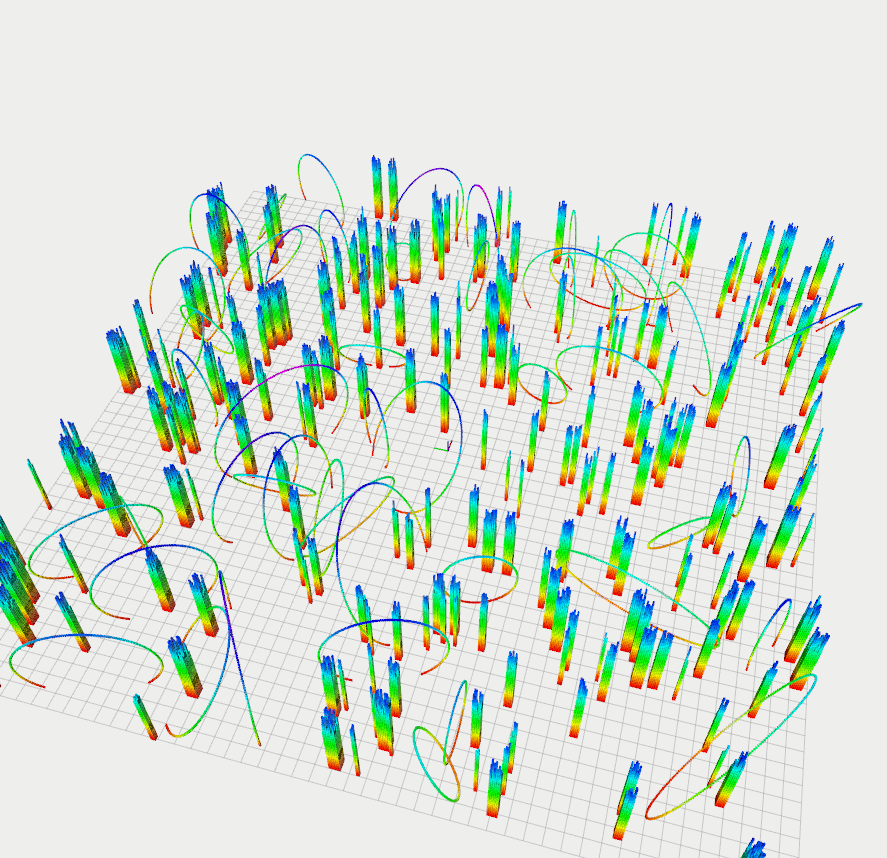
\includegraphics[width=0.3\textwidth]{random_map_overview.png}}}
    \hspace{0.2em}
    \subfigure{\label{fig:cylinder_obstacles}}\addtocounter{subfigure}{-2}
    \subfigure{\subfigure[柱形障碍物]{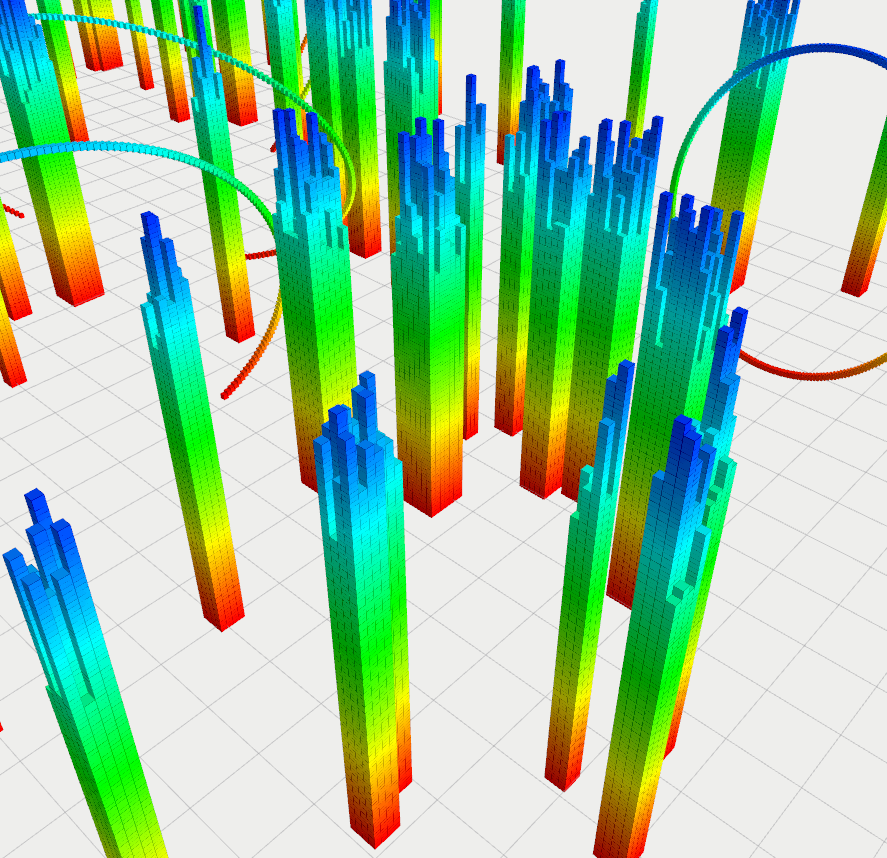
\includegraphics[width=0.3\textwidth]{cylinder_obstacles.png}}}
    \hspace{0.2em}
    \subfigure{\label{fig:circle_obstacles}}\addtocounter{subfigure}{-2}
    \subfigure{\subfigure[圆圈形障碍物]{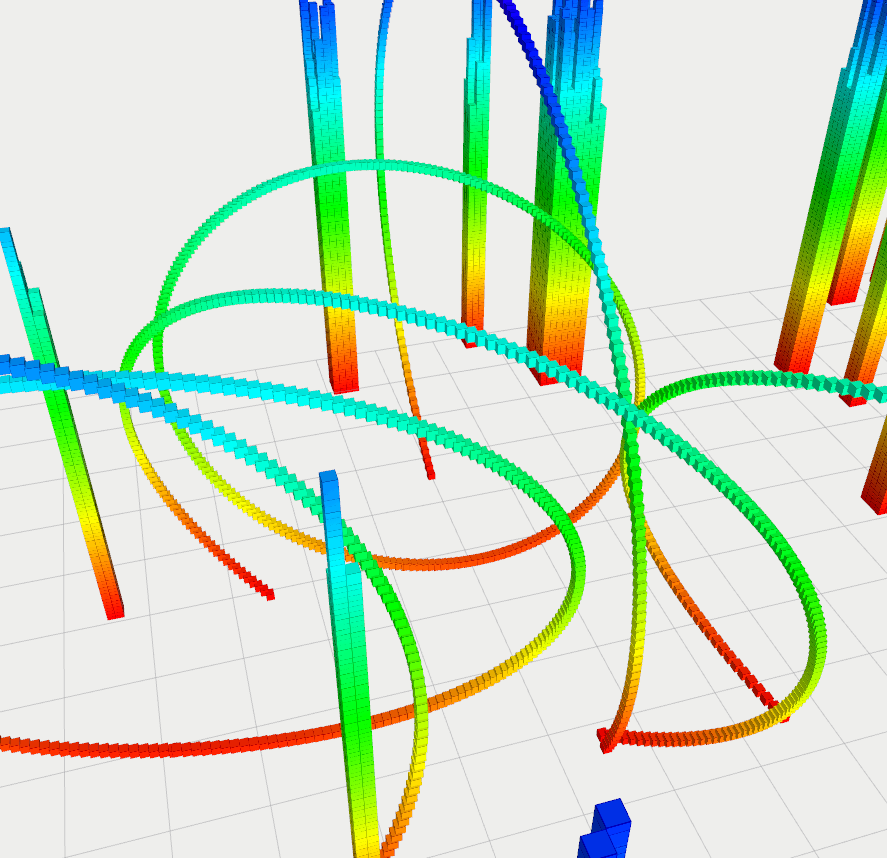
\includegraphics[width=0.3\textwidth]{circle_obstacles.png}}}
    
    \end{minipage}
    \caption{随机地图示意图}
    \label{fig:random_map}
  \end{figure}
本小节在使用现成随机地图生成程序生成的随机环境(如\figref{fig:random_map_overview}所示)中进行规划。
该程序可以根据人为指定的地图范围、障碍物数量即分辨率将障碍物随机布撒到环境中,并以点云的形式输出。
障碍物分为柱形(\figref{fig:cylinder_obstacles})和圆圈形(\figref{fig:circle_obstacles}),
二者的尺寸范围也可以人为设置

\figref{fig:random_map_planning}中分别展示了使用基于欧拉角和基于四元数两种姿态表示法在随机地图中规划出的轨迹,
轨迹多项式的次数为7(即$s=4$),
地图尺寸为50m$\times$50m,其中随机分布有300个柱形障碍物和30个圆圈形障碍物,
轨迹起始条件和终止条件中速度、加速度、加加速度以及姿态对应的RPY角均为0。

\begin{figure}[!ht]
    \setlength{\subfigcapskip}{-1bp}
    \centering
    \begin{minipage}{\textwidth}
  
    \centering
    \subfigure{\label{fig:random_map_planning_rpy}}\addtocounter{subfigure}{-2}
    \subfigure{\subfigure[基于欧拉角]{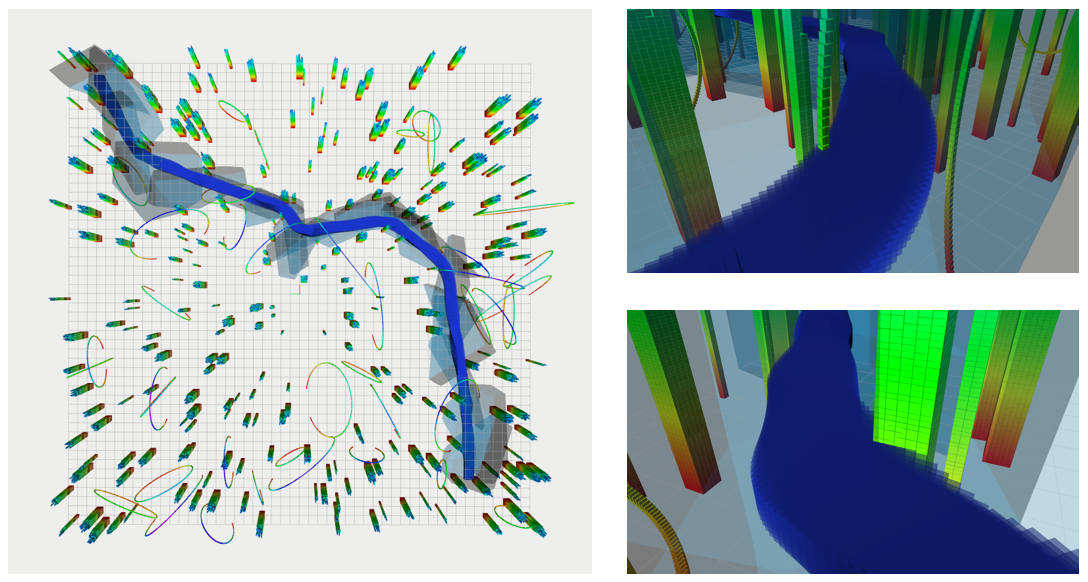
\includegraphics[width=0.88\textwidth]{random_map_rpy_planning.png}}}
    
    \subfigure{\label{fig:random_map_planning_quat}}\addtocounter{subfigure}{-2}
    \subfigure{\subfigure[基于四元数]{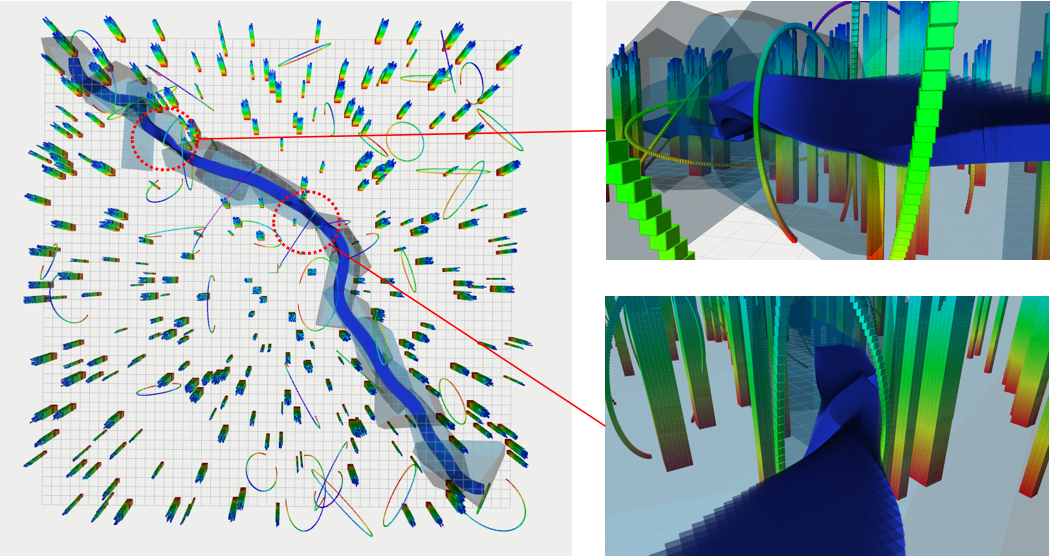
\includegraphics[width=0.88\textwidth]{random_map_quat_planning.png}}}
    
    \end{minipage}
    \caption{在随机地图中进行规划得到的轨迹及其局部细节}
    \label{fig:random_map_planning}
\end{figure}

\figref{fig:random_map_planning}中一系列半透明浅蓝色凸多面体为生成的飞行走廊,
而深蓝色带状物则是由近似表示飞行器形状的长方体组成轨迹可视化的6自由度轨迹。
可以看到,生成的轨迹均被成功约束在了安全飞行走廊内,且具有足够的平滑性。

如\figref{fig:dynamic_properties}所示分别画出了上述两条轨迹的动力学特性,
\figref{fig:dyn_prop_quat}和\figref{fig:dyn_prop_rpy}所展示的是整条轨迹中速率、加速率和角速率的变化,
红色虚线表示的是动力学限制$v_{max}$、$a_{max}$和$\omega_{max}$,
可见轨迹的动力学特性被有效地约束住了,
且在时间正则项的作用下,轨迹在大部分时间内都达到了所限制的最大速率。
\figref{fig:dyn_prop_3d_quat}和\figref{fig:dyn_prop_3d_rpy}所展示的则是速度、加速度和角速度向量的轨迹,
图中淡黄色的球所表示的则是$v_{max}$、$a_{max}$和$\omega_{max}$。

\begin{figure}[!ht]
    \setlength{\subfigcapskip}{-1bp}
    \centering
    \begin{minipage}{\textwidth}

    \centering
    \subfigure{\label{fig:dyn_prop_quat}}\addtocounter{subfigure}{-2}
    \subfigure{\subfigure[基于欧拉角法规划的轨迹动力学特性]{\includegraphics[width=0.45\textwidth]{random_map_rpy_2/dyn.png}}}
    \hspace{0.2em}
    \subfigure{\label{fig:dyn_prop_3d_quat}}\addtocounter{subfigure}{-2}
    \subfigure{\subfigure[基于欧拉角法规划的轨迹动力学特性(3D)]{\includegraphics[width=0.45\textwidth]{random_map_rpy_2/dyn_3d.png}}}

    \centering
    \subfigure{\label{fig:dyn_prop_rpy}}\addtocounter{subfigure}{-2}
    \subfigure{\subfigure[基于四元数法规划的轨迹动力学特性]{\includegraphics[width=0.45\textwidth]{random_map_quat_4/dyn.png}}}
    \hspace{0.2em}
    \subfigure{\label{fig:dyn_prop_3d_rpy}}\addtocounter{subfigure}{-2}
    \subfigure{\subfigure[基于四元数法规划的轨迹动力学特性(3D)]{\includegraphics[width=0.45\textwidth]{random_map_quat_4/dyn_3d.png}}}
    
    \end{minipage}
    \caption{所得轨迹的动力学特性示意图}
    \label{fig:dynamic_properties}
\end{figure}

上述两种规划结果的前后端相关数据如\tabref{tab:data_of_2_scenarios_in_random_map}所示。
表中数据与\figref{fig:random_map_planning}表现出了两种不同规划方式各自的典型特征,
\begin{enumerate}
    \renewcommand{\labelenumi}{(\theenumi)}
    \item 基于欧拉角的方法轨迹优化速度通常比基于四元数的方法更快;
    \item 相较基于欧拉角的方法而言,基于四元数的方法对狭小的空间和障碍无更为“敏感”:
    基于四元数的方法规划出的轨迹在穿过狭小的空间或者经过靠近障碍物的地方时更倾向于倾斜姿态来避免碰撞;
    而基于欧拉角的方法显得更为“懒惰”,常常靠近障碍物处也不会利用姿态控制来规避障碍物,所以轨迹上经常会有刮蹭发生。
\end{enumerate}

\begin{table}[htbp]
    \caption{随机地图规划两种方式前后端相关数据\label{tab:data_of_2_scenarios_in_random_map}}
    \vspace{0.5em}\centering\wuhao
    \begin{tabular}{ccccc}
    \toprule[1.5pt]
    姿态规划方式 & RRT耗时(秒) & 生成SFC耗时 & SFC凸多面体数 & 轨迹生成耗时(秒)\\
    \midrule[1pt]
    四元数 & 0.206 & 0.951 & 14 & 10.799 \\
    欧拉角 & 0.431 & 0.898 & 20 & 4.609 \\
    \bottomrule[1.5pt]
    \end{tabular}
\end{table}

首先分析优化效率的不同,考虑到两种规划方式的差异最终都体现到了罚函数$I_\Sigma$值与梯度的计算上,
\tabref{tab:analysis_of_efficiency_in_random_map_scenario}进一步给出了相关数据作对比。
其中$t_{\text{col}}$、$t_{\text{dyn}}$及$t_{\text{pen}}$分别表示单次计算碰撞惩罚项、动力学约束惩罚项以及整个罚函数的耗时。
可见在单次计算罚函数的耗时以及拟牛顿法迭代次数上四元数法均比欧拉角法更有优势,
但是最后的总优化时间却比欧拉角法要慢得多,
这说明在线搜索阶段四元数法的迭代次数远多于欧拉角法的,
于是可以推断四元数法目标函数的数值特性不利于线搜索。
至于欧拉角法以更快的速度优化出的轨迹对障碍物敏感程度不够的原因,
推测是由于欧拉角法的目标函数存在较多的局部最小值。

\begin{table}[htbp]
    \caption{随机地图规划两种方式的效率分析\label{tab:analysis_of_efficiency_in_random_map_scenario}}
    \vspace{0.5em}\centering\wuhao
    \begin{tabular}{ccccccc}
    \toprule[1.5pt]
    姿态规划方式 & $t_{\text{col}}$(毫秒) & $t_{\text{dyn}}$(毫秒)& $t_{\text{pen}}$(毫秒)& L-BFGS迭代次数 & 轨迹生成耗时(秒)\\
    \midrule[1pt]
    四元数 & 1.564 & 0.307 & 1.877 & 30 & 10.799 \\
    欧拉角 & 1.891 & 0.261 & 2.159 & 1788 & 4.609 \\
    \bottomrule[1.5pt]
    \end{tabular}
\end{table}

为更细致地研究两种不同的姿态规划方法在安全性和快速性,
本课题进一步设计了定量实验。

为衡量安全性,首先给出成功轨迹的定义:

多次规划,记录两种姿态表示法的成功率

\subsection{狭窄空间中的轨迹规划}\label{subsec:planning_in_narrow_env}

测量两种姿态表示法下计算一次罚函数所花的时间

\begin{table}[htbp]
    \caption{两种姿态规划方式在穿越狭窄缝隙的场景下的一些数据对比\label{tab:comparison_in_narrow_gap_scenario}}
    \vspace{0.5em}\centering\wuhao
    \begin{tabular}{cccccc}
    \toprule[1.5pt]
    姿态规划方式 & $t_{\text{col}}$(毫秒) & $t_{\text{dyn}}$(毫秒)& $t_{\text{pen}}$(毫秒)& L-BFGS迭代次数 & 轨迹生成耗时(秒)\\
    \midrule[1pt]
    四元数 & 0.182 & 0.055 & 0.242 & 90 & 0.838 \\
    欧拉角 & 0.230 & 0.052 & 0.286 & 2244 & 0.842\\
    \bottomrule[1.5pt]
    \end{tabular}
\end{table}

\section{仿真避障测试}\label{sec:simulation_experiments}


\section{实物避障测试}\label{sec:real_world_experiments}

\section{本章小结}\label{sec:summary_5}
